\documentclass[11pt, oneside]{article} 
\usepackage{geometry}
\geometry{letterpaper} 
\usepackage{graphicx}
	
\usepackage{amssymb}
\usepackage{amsmath}
\usepackage{parskip}
\usepackage{color}
\usepackage{hyperref}

\graphicspath{{/Users/telliott/Github/number_theory/png/}}
% \begin{center} 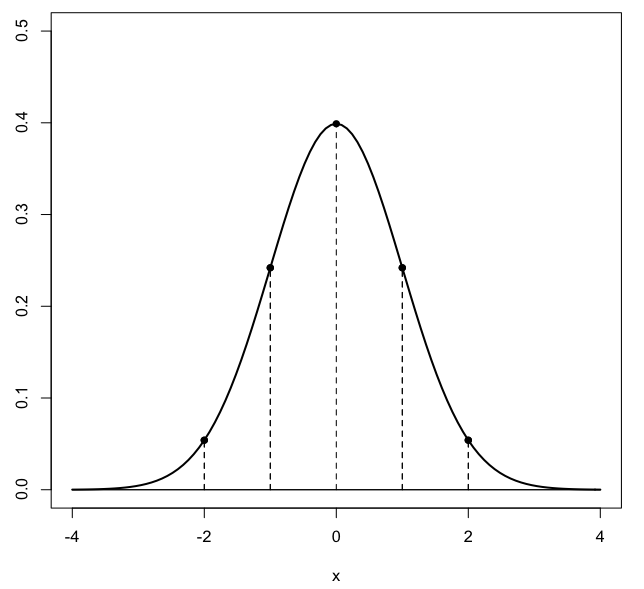
\includegraphics [scale=0.4] {gauss3.png} \end{center}

\title{Integers}
\date{}

\begin{document}
\maketitle
\Large

\subsection*{infinity is not a number}
There is a fundamental problem when we set up a division problem and $0$ is in the denominator.  What goes wrong when we attempt to divide by zero?
\[ \frac{a}{0} = \ ? \]

As we just said above, this equivalent to finding
\[ c \cdot 0 = a \]
But, by definition $c \cdot 0 = 0$.

Suppose we have $c \cdot b = a$ but $b \ne 0$, only very small.  Then, the number $c$ can get very large.  That's OK.  We can make $b$ as small as we wish by making $c$ large enough and vice versa.  But we can't say $a/0 = $ something.

If there were such a number (say $\infty$), then what about 
\[ \frac{b}{0} = \ ??  \]
\[ \frac{c}{0} = \ ??  \]

By definition, we do not allow division by zero.

And we can't answer the question what is $2 \cdot \infty$?  If we allowed multiplication by $\infty$ then the only reasonable answer would be
\[ 2 \cdot \infty = \infty \]
so then also
\[ n \cdot \infty = \infty \]
where $n$ is any number.  But then, $2 = n$.  This would be a mess.

So, by definition, \emph{infinity is not a number} and division by $0$ is \emph{undefined}.

\subsection*{limits}
Often people say that calculus is all about limits, and they are certainly where you start in proving the theoretical basis of the field.  

We will keep the discussion of limits and $\epsilon$-$\delta$ formalism to a minimum for the reasons explained in the Introduction.  But let us try to establish an intuitive idea about what we mean when we say "in the limit as $N \rightarrow \infty$".

Above we had that there is no greatest integer.

A corollary of that is the limit
\[ \lim_{n \rightarrow \infty} \frac{(n + 1) - n}{n} = 0 \]
Why?  As $n$ increases without bound, the difference between successive numbers, as a fraction of $n$, tends to zero.

To get an idea about this, first simplify by multiplying by $1/n$ on top and bottom.  Then we have
\[ \lim_{n \rightarrow \infty} \frac{(1 + 1/n - 1)}{1} = \frac{1}{n} \]

We say that $1/n$ \emph{tends} to zero as $n \rightarrow \infty$, and so does $[(n+1)-n]/n$.


\end{document}